\chapter{Introduction}
\section{Foreword}
Images and videos have acquired a big prevalence in our daily lives. From the creation of the worlds first camera, the \textit{Camera obscura}, to the creation of one of NASA's most successful science missions, the \textit{Hubble Space Telescope}, it is clear that humans have always had the urge to capture images and use them for scientific and creative purposes. Being able to create machines that can see and differentiate objects in a similar fashion to humans, has revolutionized our lives. Something as simple as recycling bottles in a supermarket is made possible by programming and utilizing techniques from image processing. Doing this enables the bottle refund machine to recognize characteristics of the bottle, rejecting or accepting it depending on the information extracted. This happens all the time wherever we go, but we rarely notice it.

One aspect of Medialogy is building systems that react accordingly to humans, to create a better human-computer confluence. For this semester project, the class was asked to focus less on the problem analysis and more on producing an entertaining product or program in which to apply knowledge taught in the Image Processing and Procedural Programming courses.


%%%%%%%%%%%%%%%%%%%%%%%% Comments for the introduction - Marta %%%%%%%%%%%%%%%%%%%%%%%%%%
% From my point of view, the introduction should be more focused on the applications of image processing, e.g. a rough explanation of what it is and what is used for in our daily life. It is ok to say that we will be using C++, but I don't see the point on commenting about the subjects that we had this semester.

%One aspect of Medialogy is building systems that react accordingly to humans. There are several technologies and theories that support this. One field in this category is called Visual Computing where Image Processing often is used, e.g. to recognize specific objects and motions. By implementing custom made software, one will be able to monitor a specific target group or process. In addition to this semester project, two mandatory courses on the third semester of Medialogy are of interest to our  project.

%The first course is called Image Processing and it is primarily based on understanding the theory of a picture and tools to manipulate the pixel values within. Knowledge such as the principle of bits and bytes, the RGB color system, histograms, and using thresholds to segment a picture, are some of the tools learned from the course. The second course used for the semester project is Procedural Programming, in which the C++ programming language was taught. The theoretical background for programming is necessary to be able to analyze and manipulate a digital image, based on theory and algorithms learned in Image Processing.

%To structure the semester projects in regards to supervisors and co-supervisors, every group was asked to discuss which subject they wanted to work with. In continuation of this every group had to submit an application for the three subjects of the biggest interest, with first, second and third priority.

Eleven topics were presented as project proposals:

\begin{itemize}
\item Image Processing for Fun utilizing an Industrial Robot
\item Image Processing for Ambient Intelligent Robots
\item Interactive Floor
\item Interactive Book
\item Interactive Drawing Game
\item Interactive Arcade Game
\item Emergency System for Old People that have fallen
\item Thermal Sock Puppet Show
\item Body Motion Controlled Exercise Game
\item Mobile App for recognizing Electric Components
\item Hj{\o}rring Library
\end{itemize}

After reading into the different project proposals, the group decided on the following three topics:

\begin{enumerate} 
\item Hj{\o}rring Library 
\item Interactive Floor 
\item Image Processing for Ambient Intelligent Robots 
\end{enumerate}

To great delight, our group was chosen to work with Hj{\o}rring Library, which was the first priority.

During the following months, the group worked on the project, which later became the \textbf{Magic Canvas}. The name is inspired by the magic of Christmas and the fact that the final project is a canvas that reflects you walking and magically turns you into a Christmas character.

\section{Establishing a collaboration with Hj{\o}rring Library}
%There were no additional predefined projects, just that it should be some kind of installation that could run at the library - preferably based on a special theme.

%A meeting was arranged with the library travelled to Hj{\o}rring to meet the library staff. Here, the group was let loose in the library to check locations for potential projects. After talking to some of the staff, more specifically our contact person Martin J{\o}rgensen, some general ideas emerged. Afterwards it was decided to go back to the university and do some initial brainstorming based on the library environment.

During the first visit to Hj{\o}rring Library, a short informational meeting was held by the staff, outlining the possibilities for the groups working at the library. Although there were no predefined projects, the staff at the library expected to get an installation that the visitors could spend some time interacting with.

The first idea that emerged included scanning barcodes from books in the library. The concept was to place a big canvas on some bookshelves and whenever people would walk past it, they would see their silhouette projected onto the canvas. The idea was that people would explore the library and depending on the books gathered and scanned, some specific graphics would appear on the canvas. This could be a hat or other clothes related to the genre of the book that was scanned. An example could be scanning a fairy tale written by H.C. Andersen which would then produce a top hat on the users head, or maybe a book with Sherlock Holmes would spawn his famous hat and pipe, etc. This would allow people that casually walk past the shelves, to see something interesting on the canvas. If they want to they could participate further by going around the library to find the correct books, scan them, and thereby change what would be projected on the canvas the next time. Maybe they would be told to find a book about Harry Potter and if they succeeded in scanning a book from the Harry Potter series, everybody walking past the canvas from now on would see themselves with a Harry Potter costume(see figure \ref{fig:bookTheme}). It seemed like a concept with endless possibilities.

\begin{figure}[htbp]
\centering
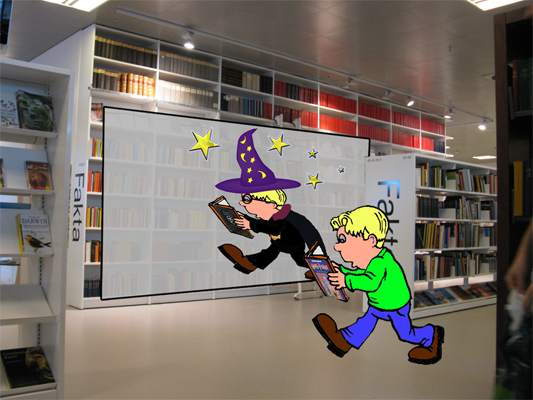
\includegraphics[width=0.7\textwidth]{Pictures/HjoerringLibrary/magician.png}
\caption{Scanning a Harry Potter book would change the theme to magic.}
\label{fig:bookTheme}
\end{figure}

After conferencing with the supervisors, it was decided that the concept needed to be narrowed down to something more specific. There were some uncertainties whether it would be possible to make a program that could track people and display graphics on top of them (e.g. a hat), as well as scan barcodes from books and extract useful data (e.g. book genre, fiction or non-fiction, etc.). Therefore it was suggested to only focus on the first part of the concept, so that instead of trying to do multiple themes we should focus mainly on one.

Another aspect that the group did not consider at first, was that the library has its own topics running for 8 to 12 weeks. The project should ideally fit into the current theme. By the time the project had to be delivered, the theme at the library was Christmas. To make the project fit the current theme, it was decided to work towards a Christmas theme.

Two members of the group then travelled to Hj{\o}rring to find a proper location for the installation. The priority was to find a spot where people would pass through naturally, instead of having to go look for the canvas. It was also necessary to check the light conditions and what equipment would be provided by the library. It was finally decided to position the installation on the walkway from the reception desk to the core of the library (see figure \ref{fig:concept_art}). This seemed to be an ideal position for the project as the lights were controllable. Also, the group was told that people tend to use that walkway either to enter or exit the library, as it is the shortest route. 

%An email was sent to Martin J{\o}rgensen from Hj{\o}rring Library describing the concept and the location we would like to use: a big bookshelf in the center of the library. Martin liked the idea, but had some concerns to identify the period in which the project would fit the library. Hj{\o}rring Library work around specific topics that change every 8-12 weeks. One of the upcoming themes at the library was Christmas, which runs from the 2nd week of November until the last week of December. Another idea then emerged in the group towards creating a project for December. Instead of working with the H.C. Andersen theme, it was decided to work with Christmas and to add a Christmas hat on top of visitors of the library. Martin was fond of this idea, and so a new meeting was arranged in order to settle on a suitable location for the project.

%Two members of the group travelled to Hj{\o}rring to participate in the meeting with Martin. The outcome was a more specific plan on the project concerning:

%\begin{itemize}
%\item The position of the project
%\item The equipment that was desired to borrow
%\item The light conditions
%\end{itemize}

%The position of the canvas was decided to be on the walkway from the reception desk to the core of the library (see figure \ref{fig:concept_art}), which Martin believed would be an ideal position for the project as the light condition is controllable. In addition to that, he knew from experience that people tend to use that walkway either to enter or exit the library, as it is the shortest route. Most importantly, it should be a place that people walk past naturally, instead of having to go out searching to find the canvas.

\begin{figure}[htbp]
\centering
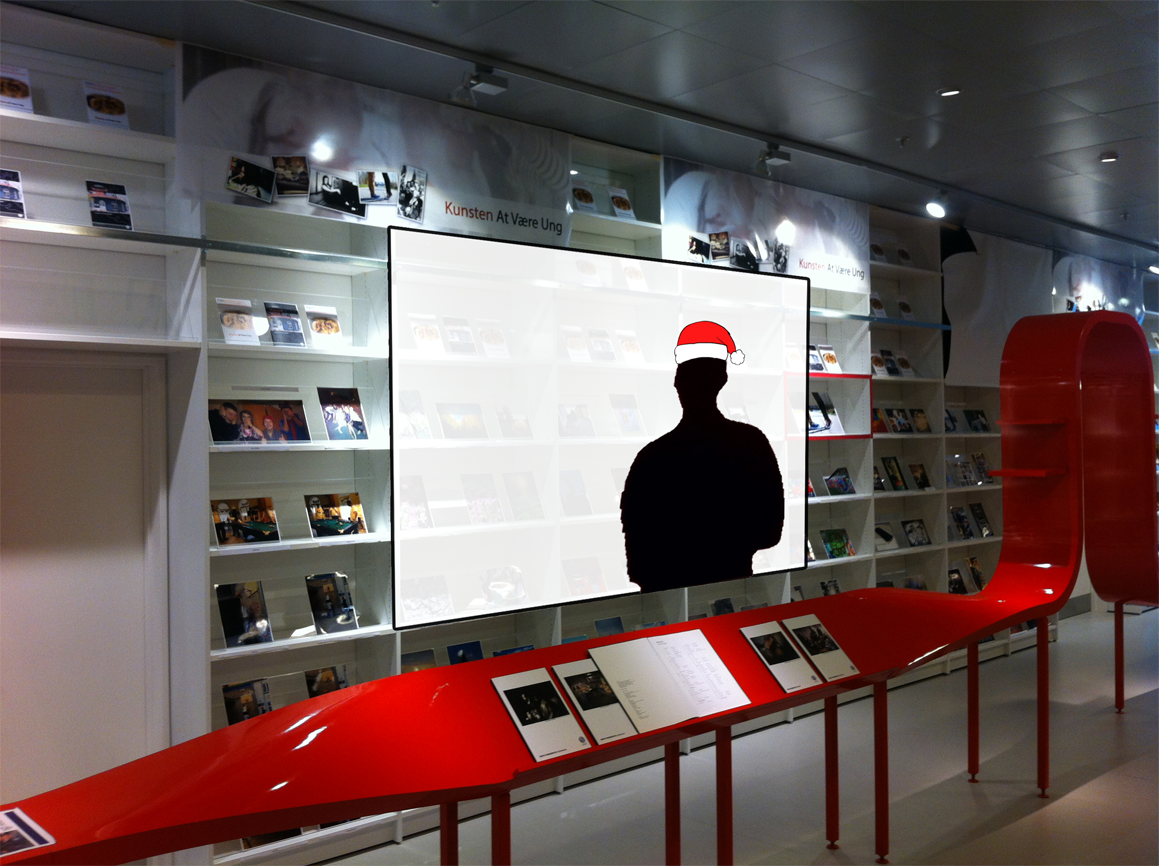
\includegraphics[width=0.7\textwidth]{Pictures/HjoerringLibrary/LocationJohannesHat.jpg}
\caption{A central location for the canvas was chosen at Hj{\o}rring Library.}
\label{fig:concept_art}
\end{figure}

%\subsection{The initial goal}

\section{Prototyping}
The first step into developing the needed software was to write some initial code that would run and produce a useful output. This was done by dividing the group into two smaller groups of three persons, with the goal of coming up with a solution on how to produce a segmentation of a video input. A competition within the group turned up to create the best code to be presented in three days. And so the "winner's code", or parts from both projects, would be incorporated in a testable file to be elaborated on in the following months.

At the end of the week, two programs were ready to be tested. Both programs were able to do the same things, only the code differed. Some of the techniques used were: median filtering; morphology (opening/closing); background subtraction; conversion from a color image to a grayscale image; and, most importantly, a first draft of the BLOB analysis that is needed to analyze the shape of the head where the Christmas hat has to be placed. All of these concepts are going to be explained more in-depth in chapter \ref{theory_part}.

The basic idea for the technical part is to have a canvas on which the shade of the visitors is projected together with the Christmas hat on the top of their head. To do this it would be necessary to have a camera gathering input about people passing by, a computer to run the program, a projector to display the output from the computer, a canvas on which the output is projected, and, lastly, controllable light conditions.

%\begin{itemize}
%\item A web camera to gather input about people walking past
%\item A computer to run the program code
%\item A projector to display the output from the computer
%\item A canvas on which the output is projected
%\item Controllable light conditions
%\item Power, cables, etc.
%\end{itemize}

\subsection{Running the first test}
As the first prototype of the program was completed, it was decided to test the code and the  equipment, to look at the video output, to test the framerate of the video and the threshold values. Figure \ref{fig:ir_cam_test} illustrates the initial setup for the first prototype testing.

\begin{figure}[htbp]
\centering
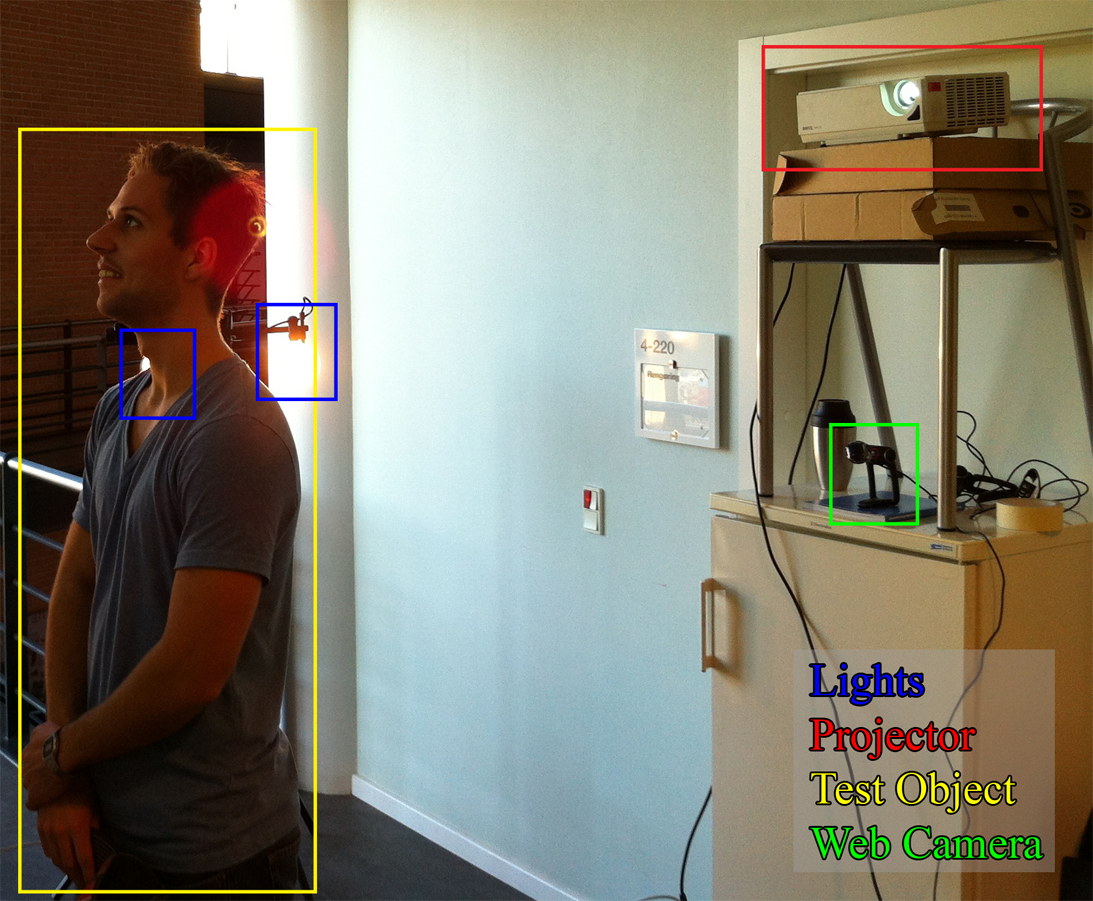
\includegraphics[width=0.80\textwidth]{Pictures/Test/TestSetup.jpg}
\caption{An early prototype test using temporary equipment.}
\label{fig:ir_cam_test}
\end{figure} 

At first a normal camera was used, but due to changes in the light conditions that came from the objects walking past, causing glitters on the output, it was decided to use a camera with an infrared filter. In addition to the infrared camera, four light bulbs were used to illuminate the person properly, so that the contrast between background and object became as big as possible. This produced a good output of the test person, but one problem still remained: once the test person faced the screen, the head was too small and didn't look very precise on the output, producing the misplacement of the Christmas hat.

The solution to this turned out to be illuminating the background instead of the person, which produced a better result, as shown in figure \ref{fig:max_subtracted}. The goal was to create as much contrast between foreground/object and background (see figure \ref{fig:max_subtracted}) as possible, and since the background is static, it seemed easier to illuminate.

\begin{figure}[htbp]
\centering
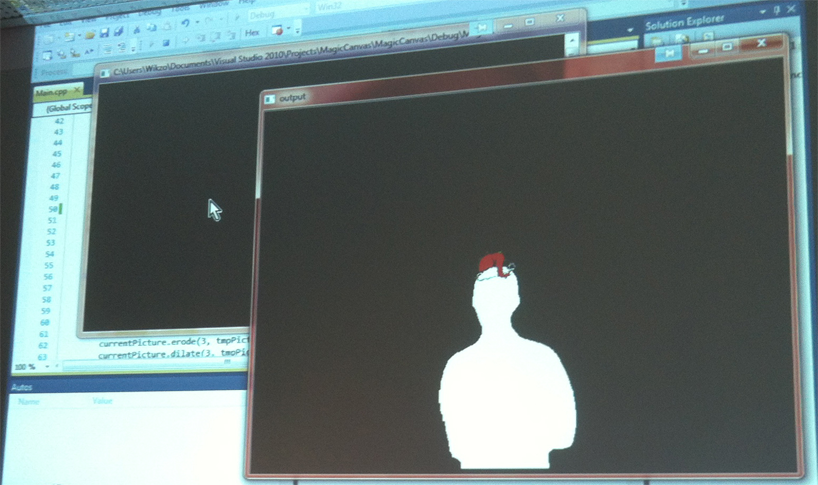
\includegraphics[width=0.80\textwidth]{Pictures/Test/MaxSubtracted.jpg}
\caption{Complete background subtraction of object outputted as binary picture. There is also some simple BLOB analysis that looks for the top-most row of pixels (the head) and displays a hat at that position.}
\label{fig:max_subtracted}
\end{figure}

\section{Changes on the main concept}
After the first short testing session it seemed clear that some things needed to be clarified. For this reason, the group asked for a brief meeting with its supervisors to receive some valuable feedback on the prototype test, as well as help with some programming dilemmas regarding speed and efficiency to loop through the big amount of pixels in each frame. At first the program code was designed to look for the top-most row of pixels, resulting on causing several different problems. The persons standing in front of the screen could end up wearing the hat on his hand just by raising it. Or it could be that somebody taller came into the picture, resulting in stealing the hat from the previous owner.

Although the group imagined the program to display the whole person as the output with a graphical hat on top, it was suggested to do not show the person directly, but instead show a shadow figure. Still, both approaches seemed to cause problems, since the program would have to loop through the whole image to find the person and then do some calculations. Even with only one person, as in the prototype test, this seemed to be a somewhat slow approach. Since the group wanted to track multiple persons, it didn't work as intended.

This dilemma were brought up and various suggestions were given, such as looking only for the head instead of the full body; adjusting the BLOB analysis to look for a more specific shape; as well as some tips on how to optimize the background subtraction.

%Considering the new information gathered, it was decided to take the project in a slightly different direction.

\subsection{Using Christmas characters instead of showing the actual person}
Instead of outputting the entire input image (the person itself) and performing several image operations, it was chosen to limit the amount of data used to find the person. Instead of looking at the whole shape, the program should only look for the head. Then it would display some pre-drawn characters underneath the head, e.g. a visitor at the library doesn't see himself, but a funny Christmas-themed character running around on the screen.

This would save a lot of calculations, as only the head of the person is of needed to be analysed. Hopefully this would lead to a more stable framerate for the program, which is important to create the proper immersion. That is why it's also relevant that the camera is quick enough to pick up and recognize new people stepping into the scene.

Another aspect to have in mind is that some people don't like to see themselves portrayed on a screen; they feel it is intimidating. But this can be easily avoided by having drawn characters instead, and it also allows a more consistent art style and the Christmas theme.
  
\section{Vision and success criteria}
The vision for the project is to make a simple, yet working program, that is fun and engaging to use at Hj{\o}rring Library. It should be something you can just walk past once and get something fun out of it, or, if you stay a little longer, you can interact with even more. It is not meant as a game per se, but more like an interactive playground where you can move around and have a good time. Another interesting aspect would be that the program should be fairly self-maintained and independent, meaning that it should need little maintenance work from the staff of the library.

Based on the above-mentioned goals of engaging people at the library, the initial vision of this semester project is to engage visitors, both passively and actively. Ultimately, the final problem statement ended being as shown in \ref{problemStatement}.

The group decided to make everything from scratch, i.e. not use any existing functionality. However, since the OpenCV library was taught in the Procedural Programming course, as well as the C++ programming language, it seemed appropriate to use it to load basic pixel information from digital images. OpenCV provides a lot of useful functionalities that could easily be used for this project, such as applying filters and looking for BLOBs, but it was chosen not to use any of those functions and write the code ourselves. This means that even though the program is going to be slower in overall terms, we don't rely on any third-party functionality.

\subsection{Problem statement}\label{problemStatement}
The group decided that in order to succeed, the final program should meet the following sets of requirements:

\begin{itemize}
\item Low maintenance: the program should be easy set up and use for the library staff.
\item Fits with the theme of Hj{\o}rring Library during December: Christmas. The program should be ready for the beginning of December.
\item It should be engaging for short periods of time, as well as for multiple uses. Multiple people should be able to use it simultaneously.
\item The program would be written in C++ and using the OpenCV library for reading/writing images, but all of the image processing functionality should be written by the group.
\end{itemize}